\toftagthis{zlutypes}
\song{Sametová}{Žlutý pes}{18pt}{1}{
\verse{1}\G{}Vzpomínám, když tehdá \C{}před lety \G{}začaly lítat \C{}rakety,\\
\G{}zdál se to bejt\C{} docela dobrej nápad\D{}. \hskip 1em \D{}\\
\G{}Saxofony hrály \C{}unyle a \G{}frčely švédský \C{}košile,\\
\G{}někdo se moh'\Em{} docela dobře \C{}flákat.\D{}

\verse{2}\textls[-25]{Když tam stál rohatej u školy, my neměli podepsaný úkoly,}\\
už tenkrát rozhazoval svoje sítě.\\
\textls[-20]{Poučen z předchozích nezdarů sestrojil elektrickou kytaru}\\
a rock'n'roll byl zrovna narozený dítě.

\chorus{}\G{}Vzpomínáš, takys tu \D{}žila a \Em{}nedělej, že jsi \C{}jiná,\\
taková \G{}malá pilná \D{}včela, taková \C{}celá\D{} sametová\G{}.

\verse{3}Přišel čas a jako náhoda byla tu bigbeatová pohoda\\
kytičky a úsmevy sekretárok.\\
Sousedovic bejby Milena je celá blbá z Boba Dylana,\\
ale to nevadí, já mám taky nárok.

\verse{4}Starý, mladý nebo pitomý mlátili do toho jako my,\\
hlavu plnou Londýna nad Temží.\\
Starej dobrej satanáš hraje u nás v hospodě mariáš,\\
pazoura se mu trumfama jenom hemží.
\clearpage
\chorus{}\G{}Vzpomínáš, už je to \D{}jinak a \Em{}jde z toho na mě \C{}zima,\\
ty jsi \G{}holka tehdá \D{}byla, taková \C{}celá\D{} sametová\G{}.

\verse{5}A do toho tenhle Gorbačov, co ho znal celej Dlabačov,\\
kopyta měl jako z Arizóny.\\
Přišel a zase odešel a nikdo se kvůli tomu nevěšel\\
a po něm tu zbyly samý volný zóny.

\chorus{}\G{}Vzpomínáš, jak jsi se \D{}měla, \Em{}když jsi nic nevě\C{}děla,\\
byla to \G{}taková krásná \D{}cela a byla \C{}celá\D{}\ldots{}\\
\G{}Vzpomínáš, jak jsi se \D{}měla, \Em{}když jsi nic nevě\C{}děla,\\
byla to \G{}taková krásná \D{}cela a byla \C{}celá\D{} sameto\G{}vá.\\
}


\toftagthis{filmove}
\song{Sandokan}{Barel Rock}{20pt}{0.95}{
\capo{3}
\verse{*}\Em{}Měl jsem hračku Igra, \Am{}plyšového \Em{}tygra,\\
on mi \D{}chcípnul, teď jsem \C{}sám, \H[7]{}rozpáral mi ho Sando\E{}kan.

\verse{1}\Em{}Italiáno seriálo, \Am{}betelné borec Sandokano,\\
\Em{}v pátek večer, v sobotu ráno \Am{}o zábavu postaráno \Em{}máš.\\
Na Momp\D{}ráčem doplul \C{}zmáčen, la Manche \D{}kanál\\
líp než \C{}Venclovský by přepla\H[7]{}val - a kdo to byl?

\chorus{}Sando\Em{}kan, Sandokan – buldo\Am{}zér do srdcí našich \Em{}dívek,\\
Sando\Em{}kan, Sandokan – \Am{}Mariana byla panna,\\
než poznala Sandokana, \Em{}joj!\\
Sandokan, Sandokan – nádherný romantický snílek,\\
Sandokan, Sandokan – míval plány velikánský\\
a pak vedl partyzánský boj.

\chorus{}Sandokan, Sandokan – chtěl bych být jako on, jako král,\\
Sandokan, Sandokan – boháčům bral, chudým dával,\\
na Mompráčem měl pak nával víc.\\
Sandokan, Sandokan – nádherný italský seriál,\\
Sandokan, Sandokan – doufám, že koupíme další díly,\\
na tu chvíli těší se nás víc.\\
}


\toftagthis{nohavica}
\song{Sarajevo}{Jaromír Nohavica}{70pt}{0.89}{
\verse{1}\Em{}Přes haličské pláně \Am[/F$\sharp$]{}vane vítr zlý,\\
to \H[7]{}málo, co jsme měli, nám \Em{}vody sebraly.\\
Jako tažní ptáci, jako rorýsi\\
letíme nad zemí, dva modré dopisy.

\chorus{}\Em{}Ještě hoří oheň a \Am{}praská dřevo,\\
\D{}ale už je čas jít \G{}spát, \H[7]{}\\
\Em{}tamhle za kopcem je \Am{}Sarajevo,\\
tam \H[7]{}budeme se zítra ráno \Em{}brát.

\verse{2}Farář v kostele nás sváže navěky,\\
věnec tamaryšku pak hodí do řeky,\\
voda popluje zpátky do moře,\\
my dva tady dole a nebe nahoře.\\
\textbf{R:}

\verse{3}Postavím ti dům z bílého kamení,\\
dubovými prkny on bude roubený,\\
aby každý věděl, že jsem tě měl rád,\\
postavím ho pevný, navěky bude stát.

\chorus{}Ještě hoří oheň a praská dřevo,\\
ale už je čas jít spát,\\
tamhle za kopcem je Sarajevo,\\
tam zítra budeme se, lásko, brát.\\
}


\toftagthis{ceskekapely}
\song{Sáro}{Traband}{30pt}{1}{
\chorus{}\Am{}Sáro, \Em{}Sáro, \F{}v noci se mi \C{}zdálo,\\
že \F{}tři andělé \C{}Boží k nám \F{}přišli na o\G{}běd.\\
Sáro, Sáro, jak moc a nebo málo\\
mi chybí abych tvojí duši mohl rozumět.

\verse{1}Sbor kajícných mnichů jde krajinou v tichu\\
a pro všechnu lidskou pýchu má jen přezíravý smích.\\
Z prohraných válek se vojska domů vrací,\\
ač zbraně stále burácí a bitva zuří v nich.\\
\textbf{R:}

\verse{2}Vévoda v zámku čeká na balkóně,\\
až přivedou mu koně, pak mává na pozdrav.\\
Srdcová dáma má v každé ruce růže,\\
tak snadno pohřbít může sto urozených hlav.\\
\textbf{R:}

\verse{3}Královnin šašek, s pusou od povidel,\\
sbírá zbytky jídel a myslí na útěk.\\
A v podzemí skrytí slepí alchymisté\\
už objevili jistě proti povinnosti lék.

\chorus{}Sáro, Sáro, v noci se mi zdálo,\\
že tři andělé Boží k nám přišli na oběd.\\
Sáro, Sáro, jak moc a nebo málo\\
ti chybí abys mojí duši mohla rozumět.

\verse{4}Páv pod tvým oknem zpívá sotva procit\\
o tajemstvích noci ve tvých zahradách.\\
A já, potulný kejklíř, co svázali mu ruce,\\
teď hraju o tvé srdce a chci mít tě nadosah!

\chorus{}Sáro, Sáro, pomalu a líně,\\
s hlavou na tvém klíně chci se probouzet.\\
Sáro, Sáro, Sáro, Sáro rosa padá ráno\\
a v poledne už možná bude jiný svět.

\F{}Sáro, \C{}Sáro, \F{}vstávej, milá \C{}Sáro,\\
\F{}andělé k nám \Dm{}přišli na \C[maj]{}oběd.\\
}


\toftagthis{folk}
\song{Sbohem, galánečko}{Vlasta Redl}{40pt}{1}{
\verse{1}\G{}Sbohem, galá\Em{}nečko, \Am{}já už musím \D{}jí - \G{}ti, \hskip 0.4em \A[7]{}\\
\D{}sbohem, galá\Hm{}nečko, \Em{}já už musím \A{}jí - \D{}ti\\
\revrpt{}\Am{} Kyselé ví\D{}nečko,\G{} kyselé ví\C{}neč\D{}ko\\
\G{}podalas mně k \C{}pi - \D{}i - \G{}tí. \rpt{}

\verse{2}\revrpt{} Sbohem, galánečko, rozlučme sa v pánu, \rpt{}\\
\revrpt{} Kyselé vínečko, kyselé vínečko\\
Podalas mně v džbánu. \rpt{}

\verse{3}\revrpt{} Ač bylo kyselé, přeca sem sa opil, \rpt{}\\
\revrpt{} eště včil sa stydím, eště včil sa stydím,\\
co jsem všechno tropil. \rpt{}

\verse{4}\revrpt{} Ale sa nehněvám, žes mňa ošidila, \rpt{}\\
\revrpt{} to ta moja žízeň, to ta moja žízeň,\\
ta to zavinila. \rpt{}\\
}


\toftagthis{anglicke}
\song{Scarborough Fair}{Simon \& Garfunkel}{45pt}{1}{
\capo{5}
\verse{1}\Am{}Are you going to \G{}Scarborough \Am{}Fair?\\
\C{} Parsley, \Am{}sage, rose\C{}ma\D{}ry and \Am{}thyme.\\
Re\Am{}member \C{}me to \C{}one \G[/H]{}who \Am{}lives \G{}there.\\
\Am{}She once \G{}was a \G{}true \Am{}love \G{}of \Am{}mine.

\verse{2}Tell her to make me a cambric shirt.\\
Parsley, sage, rosemary and thyme;\\
Without no seams nor needle work,\\
then she'll be a true love of mine.

\verse{3}Tell her to find me an acre of land.\\
Parsley, sage, rosemary and thyme;\\
Between the salt water and the sea strand,\\
then she'll be a true love of mine.

\verse{4}Tell her to reap it with a sickle of leather.\\
Parsley, sage, rosemary and thyme;\\
And gather it all in a bunch of heather,\\
then she'll be a true love of mine.

\verse{5}Are you going to\dots
}



\toftagthis{sverakuhlir}
\song{Severní vítr}{J. Uhlíř / Z. Svěrák}{30pt}{0.95}{
\verse{1}Jdu \D{}s děravou patou, mám \Hm{}horečku zlatou,\\
jsem \G{}chudý, jsem sláb, nemo\D{}cen.\\
\D{}Hlava mě pálí a \Hm{}v modravé dáli\\
se \G{}leskne a \A{}třpytí můj \D{}sen.

\verse{2} Kraj pod sněhem mlčí, tam stopy jsou vlčí,\\
tam zbytečně budeš mi psát.\\
Sám v dřevěné boudě sen o zlaté hroudě\\
já nechám si tisíckrát zdát.

\chorus{}\D{}Severní \D[7]{}vítr je \G{}krutý, \D{}počítej, lásko má, s\A[7]{} tím.\\
\D{}K nohám ti \D[7]{}dám zlaté \G{}pruty, nebo se \D{}vůbec \A[7]{}nevrá\D{}tím.

\verse{3}Tak zarůstám vousem a vlci už jdou sem,\\
už slyším je výt blíž a blíž.\\
Už mají mou stopu, už větří, že kopu\\
svůj hrob, a že stloukám si kříž.

\verse{4}Zde leží ten blázen, chtěl dům a chtěl bazén\\
a opustil tvou krásnou tvář.\\
Má plechovej hrnek a pár zlatejch zrnek\\
a nad hlavou polární zář.\\
\textbf{R:}
}


\toftagthis{arakain}
\songWithTranslation{czech}{
\song{Slečna závist}{Arakain}{15pt}{1}{
\crdheight=2.2ex

\verse{1}\Am{}Ta dívka u oltáře, co pohled tvůj teď váže,\\
skrýt \G{}závist zkouší za vlast\Am{}ním bohatstvím.\\
Má krásu, moc i slávu, přesto vidíš, že se trápí,\\
když tvář zakrývá jí závoj tkanej z černejch pavučin.\\
Áá…

\verse{2} Proč přišla takhle zrána a co si žádá u pána,\\
že svíčku drží v dlaních, tiše obchod nabízí.\\
Bože, vyslyš moje přání, jak neřekneš svý \uv{ano} mi,\\
tak ďáblu ruku podám, když mi pomoc přislíbí.\\
Áá…

\verse{3} No jen řekni, dám ti to, co chceš, já věřím, ty to dokážeš,\\
slib krví potvrdím, jen dej, ať nikdo nemá víc.\\
Mě pálí, když je kdokoli s víc štěstím, se vším, cokoliv\\
co zrovna nemám já, radši ať sama nemám nic.\\
Áá…

\verse{4}Teď otáčí se s nevolí, jak ďáblu podpis zabolí,\\
už do rysů jí kreslí vrásky z duše šedivý.\\
Pak konečně k nám promluví, skřek havraní tu zakrouží\\
a mezi námi hledá, svoji oběť vybírá.\\
Když ne mě, radši nikomu a slova nejsou k ničemu,\\
to slečna závist vstoupila zas do někoho z nás.\\
Áá…\\
}
}{english}{
\originalVersion{Lady in Black}{Uriah Heep}{0pt}{1}{
She \noprint{\Am{}}came to me one morning, one lonely Sunday morning,\\
her \noprint{\G{}}long hair flowing in the \noprint{\Am{}}mid-winter wind.\\
I know not how she found me, for in darkness I was walking\\
and destruction lay around me from a fight I could not win.\\
Ahahaaahaahah, ahahaaahahaha !

She asked me name my foe then, I said the need within some men\\
to fight and kill their brothers without thought of men or god.\\
And I begged her give me horses to trample down my enemies,\\
so eager was my passion to devour this waste of life.\\
Ahahaaahaahah, ahahaaahahaha !

But she would not think of battle that reduces men to animals,\\
so easy to begin and yet impossible to end.\\
For she, the mother of all men, had counciled me so wisely that\\
I feared to walk alone again and asked if she would stay.\\
Ahahaaahaahah, ahahaaahahaha !

\uv{Oh, lady, lend your hand,} I cried, \uv{Oh, let me rest here at your side.}\\
\uv{Have faith and trust in me,} she said and filled my heart with life.\\
\uv{There is no strength in numbers. I've no such misconceptions.\\
But when you need me be assured I won't be far away.}\\
Ahahaaahaahah, ahahaaahahaha !

Thus having spoke she turned away and though I found no words to say\\
I stood and watched until I saw her black cloak disappear.\\
My labor is no easier, but now I know I'm not alone.\\
I find new heart each time I think upon that windy day.\\
And if one day she comes to you drink deeply from her words so wise.\\
Take courage from her as your prize and say hello for me.\\
Ahahaaahaahah, ahahaaahahaha !\\
}
}


\toftagthis{nohavica}
\song{Sloní hřbitovy}{Jaromír Nohavica}{0pt}{1}{
\crdheight=2.2ex

\noexport{\textbf{Intro:}}
\vskip -8pt
\begin{figure}[h]
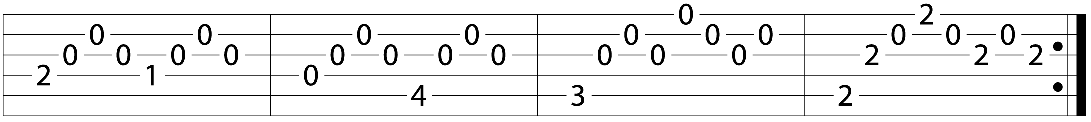
\includegraphics[width=365pt ]{res/sloni3-1.pdf}
\end{figure}
\vskip 25pt 
\begin{figure}[h]
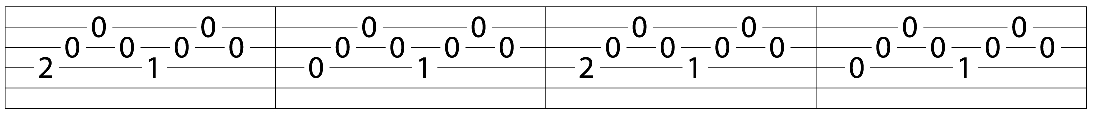
\includegraphics[width=365pt ]{res/sloni3-2.pdf}
\end{figure}
\vskip -8pt
\noprint{\Em{}}Vím o ces\noprint{\Eb[+]{}}tách, po kte\noprint{\G[/D]{}}rých chodí \noprint{\Eb[+]{}}sloni \noprint{\Em{}}pít,\noprint{\hskip 1.3em \Eb[+]{} \hskip 2.2em \G[/D]{} \hskip 2.5em \Eb[+]{}}\\
\begin{figure}[h]
\vskip 2ex
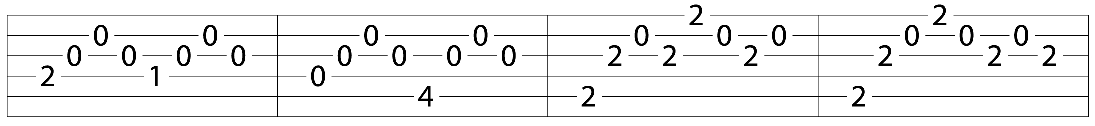
\includegraphics[width=365pt ]{res/sloni3-3.pdf}
\vskip -2ex
\end{figure}
\noprint{\Em{}}jsou žízní \noprint{\Eb[+]{}}rozryté, \noprint{\G[/D]{}}váhám, zda \noprint{\Db[dim]{}}dál mám \noprint{\H[7]{}}jít.\noprint{\hskip 2em \H[7]{}}\\
\begin{figure}[h!]
\vskip 2ex
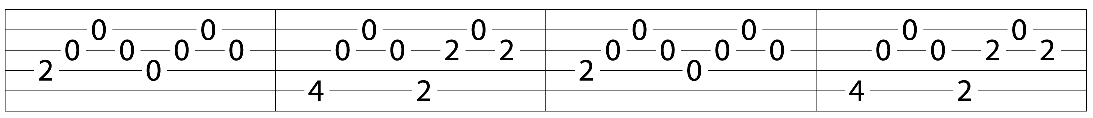
\includegraphics[width=365pt ]{res/sloni3-4.pdf}
\vskip -2ex
\end{figure}
\textls[-10]{\noprint{\Em{}}Na konci \noprint{\G[/D]{}}nečeká tů\noprint{\Db[dim]{}}ň s vodou \noprint{\H[7]{}}spásnou, \noprint{\\}\noprint{\Em{}}na konci \noprint{\G[/D]{}}poslední\noprint{\Db[dim]{}} naděje \noprint{\hskip 1em\H[7]{}}zhasnou,}\\
\begin{figure}[h!]
\vskip 2ex
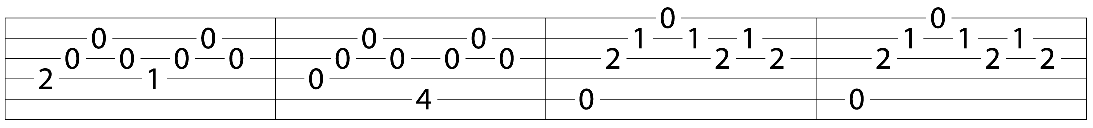
\includegraphics[width=365pt ]{res/sloni3-5.pdf}
\vskip -2ex
\end{figure}
už \noprint{\Em{}}vím, kde \noprint{\Eb[+]{}}leží \noprint{\hskip 1em \G[/D]{}}sloní \noprint{\hskip 1em\Db[dim]{}}hřbitov, \noprint{\\}\noprint{\Am{}}vím, kde najdeš kosti sluncem \noexport{\\}
\begin{figure}[h!]
\vskip 2ex
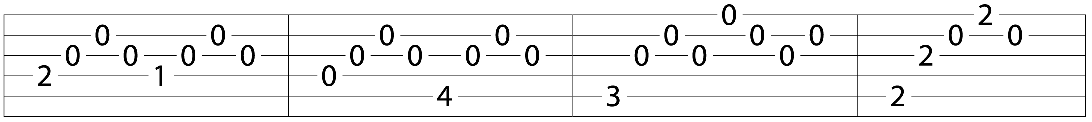
\includegraphics[width=365pt ]{res/sloni3-7.pdf}
\vskip -2ex
\end{figure}
\noprint{\Em{}}vyprah\noprint{\CHORD{\dots}{}}lé\ldots{}

\clearpage
\begin{figure}[h!]
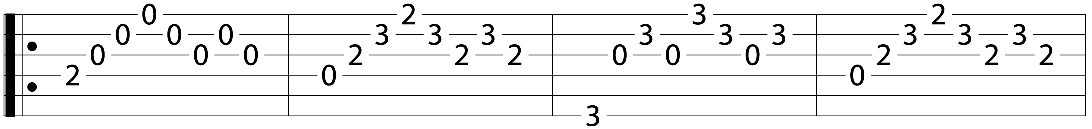
\includegraphics[width=365pt ]{res/sloni3-8.pdf}
\vskip -2ex
\end{figure}
Až nám \noprint{\Em{}}hvězdy přestanou \noprint{\D{}}svítit, až nám \noprint{\G{}}slunce přestane \noprint{\D{}}hřát,\\
\begin{figure}[h!]
\vskip 2ex
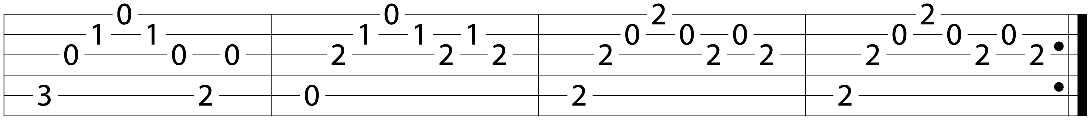
\includegraphics[width=365pt ]{res/sloni3-9.pdf}
\vskip -2ex
\end{figure}
až se \noprint{\C{}}budeme vesmírem \noprint{\Am{}}řítit, napo\noprint{\H[7]{}}řád\ldots{}\\
\begin{figure}[h!]
\vskip 2ex
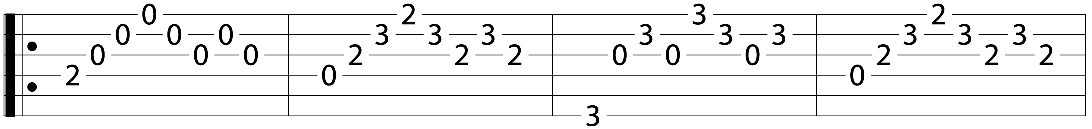
\includegraphics[width=365pt ]{res/sloni3-8.pdf}
\vskip -2ex
\end{figure}
Až mi \noprint{\Em{}}hvězdy přestanou \noprint{\D{}}svítit, až mi \noprint{\G{}}slunce přestane \noprint{\D{}}hřát,\\
\begin{figure}[h!]
\vskip 2ex
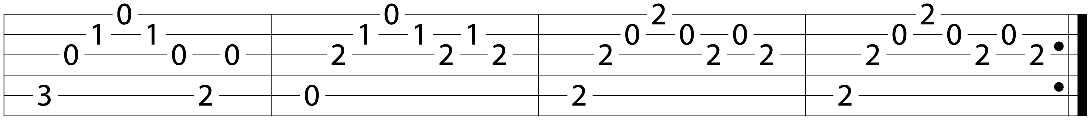
\includegraphics[width=365pt ]{res/sloni3-9.pdf}
\vskip -2ex
\end{figure}
chci se \noprint{\C{}}s vámi vesmírem \noprint{\Am{}}řítit, napo\noprint{\H[7]{}}řád,\noexport{\\}
\begin{figure}[h!]
\vskip 2ex
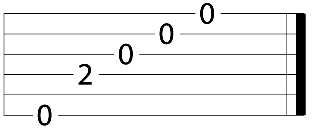
\includegraphics[scale=0.65 ]{res/sloni3-10.pdf}
\vskip -2ex
\end{figure}
napo\noprint{\Em{}}řád.
}
\Large
\crdheight=2.2ex
\toftagthis{filmove}
\song{Slunečný hrob}{Blue Effect}{35pt}{0.80}{
\rec{Usínám a chtěl bych se vrátit\\
o nějakej ten rok zpátky,
bejt zase malým klukem,\\
kterej si rád hraje a~který je s tebou.}

\vskip -1ex
\leftskip 70pt
\verse{1}\E{}Zdá se \Fsm{}mi, \hskip 1em \Gsm{} je to \hskip 0.4em \Fsm{}moc let,\\
já byl kluk, kterej chtěl\\
znáti svět, s tebou jsem si hrál.\\
\verse{*}\textbf{\sffamily G6 \hskip 0.5em F$\sharp$7 \hskip 0.5em Fmaj7}

\verse{2}Vrátím se a chtěl bych rád\\
být s tebou, zavzpomínat,\\
\E{}mám tu \Fsm{}teď \hskip 1em \Gsm{} ale \hskip 1em \Fsm{}zprávu \E{}zlou\E{}. \hskip 1em \E[7]{} \hskip 1.8em \E[7]{}

\chorus{}\Csm{}Su \hskip 0.3em - \hskip 0.3em \Dsm{}chá \hskip 1em \A{}hlína \Gsm{}ta - dy, \hskip 0.2em \Fsm{}\\
bez kvítí, bez vody,\\
\Gsm{} já na ni \Fsm{}poklekám,\\
\Gsm{}vzpomínkou po\H{}cta se vzdává.

\verse{3}Loučím se a něco však\\
tam zůstalo z těch našich dnů,\\
já teď vím, věrný zůstanu.\\
\textbf{R:}

\vskip -1ex
\verse{4}Loučím se\dots

\leftskip 35pt
\rec{Nemohu spát, probouzím se a zase se nemohu ubránit\\ myšlence,vrátit se o nějakej ten rok zpátky, bejt zase\\
malým klukem, kterej si rád hraje, který je s \emph{\E[9]{}}tebou.}
}



\toftagthis{olympic}
\song{Slzy tvý mámy}{Olympic}{20pt}{1}{
\capo{3}
\verse{1}\Em{}Chvilku vzpomínej,\Am{} je to všechno jen pár let,\\
\D{}na kytaru v duchu hrej,\G{} tvoje parta \G[/F$\sharp$]{}je tu hned.\\
\Em{}Z cigaret je modrej dým, \E[7]{}hraje magneťák,\\
\Am{}holka sedla na tvůj klín, \Em{}nevíš ani \Hm{}jak,\\
nevíš \Em{}jak.\hskip 1em \D{} \hskip 1em \Em{} \hskip 2em \D{}

\verse{2}Tvý roky bláznivý chtěly křídla pro svůj let,\\
dnes už možná nevíš sám, proč tě tenkrát pálil svět.\\
Chtěl jsi prachy na mejdan, byl to hloupej špás,\\
když jsi v noci vyšel ven, snad ses trochu třás, trochu třás.

\verse{*}\E{}Když tě našel noční \D{}hlídač,\\
byl by \C{}to jen příběh \G{}bláznivýho kluka,\\
\C{}nebejt nože \G{}ve tvejch dětskej rukách,\\
\C{}nebejt strachu \G{}mohlo to bejt \D{}všechno \Em{}jináč.\H[7]{}

\chorus{}\Em{}Slzy tvý mámy \D{}šedivý \Hm{}stékají na \Em{}polštář,\\
\C{}kdo tě zná, se vůbec \D{}nediví, že stárne \G{}její tvář.\H[7]{}\\
\Em{}Nečekej úsměv od ženy, který jsi \Am{}všechno vzal,\Am[/G]{}\\
jen pro tvý \Em{}touhy zborcený, \D{}léta ztrace\Hm{}ný,\\
ty oči \Em{}pláčou dál.

\verse{3}Když jsi vyšel ven, ze žalářních vrat,\\
možná, že jsi tenkrát chtěl znovu začínat.\\
Poctivejma rukama, jako správnej chlap,\\
snad se někdo ušklíb jen,\\
že jsi křivě šláp, křivě šláp.

\verse{*}I když byl někdo k tobě krutej,\\
proč jsi znovu začal mezi svejma,\\
tvůj pocit křivdy se pak těžko smejvá,\\
když hledáš vinu vždycky jenom v druhejch.\\
\textbf{R:}

}


\toftagthis{spiritual}
\song{Soudný den}{Spirituál kvintet}{55pt}{1}{
\verse{1}\Am{}Zdál se mi sen, že se nebe hroutí,\\
\G{}zdál se mi sen o poslední pouti,\\
\Am{}zdál se mi sen, že všechno seberou ti\\
v ten \Em{}soudný \Am{}den.

\verse{2}Kam běžet mám, Slunce rychle chladne,\\
kam běžet mám, měsíc na zem spadne,\\
kam běžet mám, moře už je na dně\\
v ten soudný den.

\verse{3}Stůj, nechoď dál, času už je málo,\\
stůj, nechoď dál, míň, než by se zdálo,\\
stůj, nechoď dál, otevři se, skálo,\\
v ten soudný den.

\verse{4}Pán tě zavolá, má pro každého místo,\\
Pán tě zavolá, jen kdo má duši čistou,\\
Pán tě zavolá, sám nedokázal bys to\\
v ten soudný den.

\verse{5}Soudí, soudí pány, slouhy,\\
soudí, soudí hříšné touhy,\\
\Am{}soudí, soudí, výčet pouhý, \Am{}á\ldots \hskip 0.5em  \A[sus2]{} \hskip 3em \E[sus4]{} \hskip 3em \E{}

\verse{*}\Am{}Vtom se probudíš, to byl jen sen,\\
\F{}vtom se probudíš, to byl jen sen,\\
\Dm[6]{}vtom se probudíš, to byl jen sen,\\
\Am{}jen \hskip 1em \E{}pouhý \Am{}sen.

\verse{6} Zdál se mi sen, že se nebe hroutí \dots

\verse{7}Zdál se mi sen, já stojím na svém místě,\\
zdál se mi sen, mé svědomí je čisté,\\
\Am{}zdál se mi sen, jen jedno vím \F{}jistě:\\
\Am{} je \hskip 1em  \E{}soudný \Am{}den!
~\\}


\toftagthis{anglicke}
\song{Sound of Silence}{Simon \& Garfunkel}{45pt}{1}{
\capo{6}
\verse{1}\Am{}Hello darkness, my old \G{}friend,\\
I've come to talk with you \Am{}again,\\
because a vision softl\F{}y cree\C{}ping\\
left its seeds while I w\F{}as slee\C{}ping\\
and the \F{}vision that was planted in my \C{}brain\\
still re\C{}mains\Am{}\\
\C{}within the \G{}sound of \Am{}silence.

\verse{2}In restless dreams I walked alone,\\
narrow streets of cobblestone.\\
'Neath the halo of a street lamp,\\
I turned my collar to the cold and damp,\\
when my eyes were stabbed by\\
the flash of a neon light,\\
that split the night\\
and touched the sound of silence.

\verse{3}And in the naked light I saw\\
ten thousand people, maybe more.\\
People talking without speaking,\\
people hearing without listening,\\
people writing songs that voices never share\\
and no one dared\\
disturb the sound of silence.

\verse{4}\uv{Fools,} said I, \uv{You do not know,\\
silence like a cancer grows.\\
Hear my words that I might teach you,\\
take my arms that I might reach you.}\\
But my words like silent raindrops fell\\
and echoed in the wells of silence

\verse{5}And the people bowed and prayed\\
to the neon god they made.\\
And the sign flashed out its warning\\
in the words that it was forming.\\
And the sign said: `The words of the prophets\\
are written on the subway walls\\
and tenement halls\\
and whispered in the sound of silence.'\\
}


%\toftagthis{anglicke}
%\song{Stairway to Heaven}{Led Zeppelin}{10pt}{1}{
%\vskip 8pt
%\verse{1}There's a lady who's sure, all that glitters is gold\\
%and she's buying a stairway to heaven.\\
%\textls[-17]{When she gets there she knows, if the stores are all closed}\\
% with a word she can get what she came for.\\
% Ooh, ooh, and she's buying a stairway to heaven.
%
%\verse{2}There's a sign on the wall but she wants to be sure,\\
% 'cause you know sometimes words have two meanings.\\
% In a tree by the brook, there's a songbird who sings,\\
% sometimes all of our thoughts are misgiven.
%
% Ooh, it makes me wonder,\\
%ooh, it makes me wonder.
%
%\verse{3}There's a feeling I get when I look to the west\\
%and my spirit is crying for leaving.\\
%\textls[-25]{In my thoughts I have seen rings of smoke through the trees}\\
%and the voices of those who stand looking.
%
% Ooh, it makes me wonder,\\
% ooh, it really makes me wonder.
%
%\verse{4}And it's whispered that soon, if we all call the tune,\\
% then the piper will lead us to reason.\\
% And a new day will dawn for those who stand long,\\
%and the forests will echo with laughter.
%\clearpage
%\verse{5}\textls[-15]{If there's a bustle in your hedgerow, don't be alarmed now,}\\
% it's just a spring clean for the May queen.\\
%\textls[-15]{Yes, there are two paths you can go by, but in the long run}\\
% there's still time to change the road you're on.\\
% And it makes me wonder.
%
%\verse{6}\textls[-45]{Your head is humming and it won't go, in case you don't know,}\\
% the piper's calling you to join him.\\
%\textls[-15]{Dear lady, can you hear the wind blow and did you know}\\
%your stairway lies on the whispering wind?
%
%\verse{7} And as we wind on down the road,\\
% our shadows taller than our soul.\\
%There walks a lady we all know,\\
%who shines white light and wants to show,\\
%how everything still turns to gold\\
%and if you listen very hard,\\
%the tune will come to you at last,\\
%when we all are one and one is all,\\
%to be a rock and not to roll.
%
% And she's buying the stairway to heaven.\\
%}


\toftagthis{anglicke}
\song{Stand By Me}{Ben E. King}{30pt}{1}{
\verse{1}When the \A{}night has come\Fsm{} and the land is dark\\
and the \D{}moon is the \E{}only light we'll \A{}see,\\
no I won't be afraid, oh, I won't be afraid,\\
just as long as you stand, stand by me.

\chorus{}So darling, darling,\\
stand by me, oh stand by me,\\
oh stand, stand by me, stand by me.

\verse{2}If the sky that we look upon should tumble and fall,\\
all the mountains should crumble to the sea,\\
I won't cry, I won't cry, no, I won't shed a tear,\\
just as long as you stand, stand by me.

\chorus{}And darling, darling,\\
stand by me, oh stand by me,\\
oh stand now, stand by me, stand by me.

\chorus{}So darling, darling,\\
stand by me, oh stand by me,\\
oh stand now, stand by me, stand by me.\\
Whenever you're in trouble won't you stand by me,\\
oh stand by me, oh won't you stand now, stand,\\
stand by me\\
}


\toftagthis{spiritual}
\song{Stará archa}{Spirituál kvintet}{60pt}{0.9}{
\chorus{}\revrpt{} Já mám \D{}kocábku náram-, \A[7]{}náram-, \D{}náram-,\\
kocábku náram-, \A[7]{}náram\D{}nou. \rpt{}

\verse{1}\D{}Pršelo a blejskalo se sedm neděl,\\
kocábku náram-, \A[7]{}náram\D{}nou,\\
Noe nebyl překvapenej, on to věděl,\\
kocábku náram-, \A[7]{}náram\D{}nou.\\
\textbf{R:}

\verse{*}\D{}Archa má cíl, archa má směr,\\
plaví se k Araratu \A[7]{}na se\D{}ver.\\
\textbf{R:}

\verse{2}Šem, Nam a Jafet byli bratři rodní,\\
kocábku náram-, náramnou,\\
Noe je zavolal ještě před povodní,\\
kocábku náram-, náramnou.

\verse{3}Kázal jim naložiti ptáky, savce,\\
kocábku náram-, náramnou.\\
\uv{Ryby nechte, zachrání se samy hladce,}\\
kocábku náram-, náramnou.\\
\textbf{R:, *., R:}

\verse{4}Přišla bouře, zlámala jim pádla, vesla,\\
kocábku náram-, náramnou,\\
tu přilétla holubice, snítku nesla,\\
kocábku náram-, náramnou.

\verse{5}Na břehu pak vyložili náklad celý,\\
kocábku náram-, náramnou,\\
ještě že tu starou dobrou archu měli,\\
kocábku náram-, náramnou.\\
\textbf{R:, *., R:, R:}\\
}

\toftagthis{spiritual}
\song{Starý příběh}{Spirituál kvintet}{50pt}{0.89}{
\verse{1}Řek' \D{}Mojžíš jednou lidu svému: Přišel čas,\\
dnes v noci tiše \Fsm{}vytratí se \G{}každý \A[7]{}z vás,\\
\D{}mává\D[7]{}, \hskip 1em \G{}mává\Gs[dim]{} \hskip 1em nám \D{}všem \A[7]{}svobodná \D{}zem.

\verse{2}Já říkám rovnou, každý ať s tím počítá,\\
že naše cesta ke štěstí je trnitá,\\
mává, mává nám všem svobodná zem.\\
\chorus{}\revrpt{} A \D{}kdo se bojí vodou jít,\\
ten podle tónů faraónů musí \A[7]{}žít,\\
\D{}mává\D[7]{}, \hskip 1em  \G{}mává\Gs[dim]{} \hskip 1em  nám \D{}všem \A[7]{}svobodná \D{}zem. \rpt{}

\verse{3}Až první krůček bude jednou za námi,\\
už nikdo nesmí zaváhat, dát na fámy,\\
mává, mává nám všem svobodná zem.

\verse{4}Pak tenhle vandr všem potomkům ukáže,\\
že šanci má jen ten, kdo má dost kuráže,\\
mává, mává nám všem svobodná zem.\\
\textbf{R:}

\verse{5}Ten starý příběh z bible vám tu vykládám,\\
ať každý ví, že rozhodnout se musí sám,\\
mává, mává nám všem svobodná zem.\\
\textbf{R:}\\
}

\toftagthis{nedvedi}
\song{Stánky}{Nedvědi}{55pt}{1}{
\verse{1}\D{}U stánků \G{}na levnou krásu,\\
\D{}postávaj' a \Gm{}smějou se času\\
\D{}s cigaretou a \A[7]{}s holkou, co nemá kam j\D{}ít.

\verse{2}Skleniček pár a pár tahů z trávy,\\
uteče den, jak večerní zprávy,\\
neuměj' žít a bouřej' se a neposlouchaj'.

\chorus{}\D[7]{} Jen\G{} zahlídli svět, maj' \A[7]{}na duši vrásky,\\
tak \D{}málo je, tak \Gm{}málo je lásky,\\
\D{}ztracená víra \A[7]{}hrozny z vinic neposbír\D{}á.

\verse{3}U stánků na levnou krásu,\\
postávaj' a ze slov a hlasů\\
poznávám, jak málo jsme jim stačili dát.\\
\textbf{R: $(2\times)$}\\
}


\song{Stín katedrál}{Karel Svoboda}{40pt}{1}{
\verse{1}\A{}Stín \D{}katedrál, \A{}půl nebe s bůhví \G{}čím, \D{}jé \E{}jé,\\
\A{}svůj \D{}ideál, \A{}sen, co si \H[7]{}dávám \E{}zdát.\E[7]{}\\
Z úsměvů šál, dům nebo básní rým, jéjé\\
jé, co ti dál, mám, řekni, dárkem dát.

\chorus{}\C{}Přej si, co \D{}chceš, zlatý \G{}důl nebo \D{}věž,\\
sladkou \C{}sůl, smutný \D{}ráj, suchý \G{}déšť. \G{}\\
\C{}Ber, tady \D{}máš mořskou \G{}pláň nebo \D{}pláž,\\
hudbu \C{}sfér, jenom \D{}ber se mnou \E{}též, \Hm[7]{}jé \hskip 1.8em \E[7]{}jé.

\verse{2}\A{}Můj \D{}ideál, \A{}víš, to co já mám \G{}rád, \D{}jé \E{}jé,\\
\A{}stín \D{}katedrál, \A{}sen, co si \H[7]{}k ránu \D{}dá - \E[7]{}vám \A{}zdát.\\
\textbf{R:}

\verse{3} Můj ideál, víš \dots

\revrpt{} \H[7]{}Sen, co se \E{}nám bude \A{}zdát. \rpt{}\\
}


\toftagthis{anglicke}
\song{Suicide is Painless}{M*A*S*H theme}{60pt}{1.05}{
\vskip 8pt
\verse{1}Through \Dm[7]{}early morning \G[7]{}fog I see\\
\C[maj]{}visions of the \Am[7]{}things to be,\\
the \Dm[7]{}pains that are with\G[7]{}held for me,\\
I \C{}realize and \Am[7]{}I can see\A[7]{}.

\chorus{}That \Dm[7]{}suicide is \G[7]{}painless,\\
it \C[maj]{}brings on many \Am[7]{}changes\\
and \F[maj]{}I can \Am{}take or \Dm[7]{}leave it \G[7]{}if I \Am{}please.

\verse{2}Try to find a way to make\\
all our little joys relate\\
without that ever present hate,\\
but now I know that it's too late.\\
And\ldots{}+ \textbf{R:}

\verse{3}The game of life is hard to play,\\
I'm going to lose it anyway,\\
the losing card I'll someday lay,\\
so this is all I have to say.\\
That\ldots{}+ \textbf{R:}
\clearpage
\verse{4}The only way to win is cheat\\
and lay it down before I'm beat\\
and to another give a seat\\
for that's the only painless feat.\\
'Cause\ldots{}+ \textbf{R:}

\verse{5}The sword of time will pierce our skins,\\
it doesn't hurt when it begins,\\
but as it works it's way on in,\\
the pain grow stronger watch it grin.\\
For\ldots{}+ \textbf{R:}

\verse{6}A brave man once requested me\\
to answer questions that are key,\\
is it to be or not to be\\
and I replied \uv{Oh, why ask me.}\\
'Cause\ldots{}+ \textbf{R:}

And you can do the same thing if you please.\\
}


\toftagthis{ceskekapely}
\song{Svařák}{Harlej}{50pt}{1}{
\verse{1}\G{}Když jsem sám doma, \Am{}poslouchám Vávra,\\
\C{}starýho vola, \D{}pořád dokola.\\
\G{}Chce to mít nápad, \Am{}a né pořád chrápat,\\
\C{}já dostal jsem nápad, \D{}udělat mejdan.

\chorus{}Mám \G{}rád svařené \Am{}víno červené,\\
já mám \C{}rád, rád sva\G{}řák.\\
Mám \G{}rád svařené \Am{}víno červené,\\
já mám \C{}rád, rád sva\G{}řák.

\verse{2}Se známou partou, domluva krátká,\\
zejtra v 6 hodin, vstup jedna lampa.\\
Začíná mejdan, na 200 \%,\\
my plníme plány, rostou nám blány.\\
\textbf{R: $(2\times)$}\\
}



\toftagthis{ceskekapely}
\song{Svaz českých bohémů}{Wohnout}{20pt}{1}{
\capo{1}
\medskip
\chorus\E{}Vracím se domů nad rá\Hm{}nem, kvalitním vínem omá\Fsm{}men,\\
z přímek se stávaj zatá\D{}čky, točí se \A{}svět, jsem na sra\E{}čky.\\
Vedle mě zvrací princezna, nastavím dlaň a požehnám,\\
pro všechny jasný poselství - tomu se říká přátelství. 

\verse{1}Mám tisíc otázek na žádnou vzpomínku,\\
skládám si obrázek kámen po kamínku.\\
Včerejší produkce šla do bezvědomí,\\
nastává dedukce, co na to svědomí. 

\verse{2}A už si vzpomínám, já byl jsem na srazu,\\
s kumpány který mám, patříme do svazu,\\
vlastníme doménu, tak si nás rozklikni,\\
svaz českejch bohémů\dots{}\\
\textbf{R:}

\verse{3}Stačí pár večírků, společně s bohémy,\\
za kterými se táhnou od školy problémy.\\
V partě je Blekota, Jekota, Mekota,\\
dost často hovoříme o smyslu života.

\verse{4}Jako je třeba teď, mám tisíc otázek,\\
na žádnou vzpomínku, si skládám obrázek.\\
Z těžkejch ran lížu se, včera jsme slavili,\\
svatýho Vyšuse.\\
\textbf{R:}\\

\verse{5}Svět zrychluje svý otáčky, sousedka peče koláčky.\\
Hlášen stav nouze nejvyšší, Hapkové volaj Horáčky.\\
Zástupy českejch bohému, vyráží ven do terénů\\
šavlí z kvalitního vína bojovat proti systému.

\revrpt{} Tak jsme se tu všichni sešli, co myslíš, osobo?\\
Na to nelze říci než \uv{Co je ti do toho?}\\
Tak jsme se tu všichni sešli, co myslíš, osude?\\
Na to nelze říci než \uv{Jinak to nebude.} \rpt\\
}


\toftagthis{anglicke}
\song{Sweet Home Alabama}{Lynyrd Skynyrd}{25pt}{0.93}{
\verse{1}\D{}Big \C{}wheels keep on \G{}turning,\G{}\\
carry me home to see my kin.\\
Singing songs about the Southland,\\
I miss Alabamy once again and I think it's a sin.

\verse{2}Well I heard mister Young sing about her,\\
well, I heard old Neil put her down.\\
Well, I hope Neil Young will remember,\\
a Southern man don't need him around anyhow.

\chorus{}Sweet home Alabama,\\
where the skies are so blue.\\
Sweet Home Alabama,\\
\D{}Lord, I'm \C{}coming home to \G{}you. \F{} \hskip 1em \C{}

\verse{3}In Birmingham they love the governor, \F{}boo \C{}hoo \D{}hoo!\\
Now we all did what we could do,\\
now Watergate does not bother me,\\
does your conscience bother you? Tell the truth.\\
\textbf{R:}

\verse{4}Now Muscle Shoals has got the Swampers\\
and they've been known to pick a song or two,\\
Lord, they get me off so much,\\
they pick me up when I'm feeling blue,\\
now how about you?\\
\textbf{R: $(2\times)$}
}


\toftagthis{hapka}
\song{Šaškové počmáraní}{Petr Hapka / Michal Horáček}{70pt}{1}{
\verse{1}\C{}Koukněte na toho \H[7]{}fintila,\\
\Dm{}pod krkem žlutého \G[7]{}motýla,\\
\Dm{}zelený klobouček \G[7]{}do týla\\
\D[7]{}šoupne si \G[7]{}na bílou \C{}pleš. \G[+]{}

\verse{2}I když ten tralalák padá mi,\\
hlavně že vyhrávám barvami,\\
hlavně že vyhrávám barvami,\\
\D[7]{}zase jsem \G[7]{}šťastnej jak \C{}veš.\C[7]{}

\chorus{}Co po mně \F{}chceš, pravdu či \Fm{}lež?\\
Zkus ty dvě \C{}rozeznat a pak se \C[7]{}směj,\\
barevný \F{}svět láme mi \Fm{}hřbet,\\
\Em{}přesto chci být \Eb[dim]{}šašek \hskip 0.7em \Dm[7]{}počmára\G[7]{}nej.

\verse{3}Ucho mi hryžou jak oplatku,\\
s rozběhem kopou mě do zadku,\\
tvrděj, že všechno je v pořádku,\\
když mi daj' mizernej plat.

\clearpage
\verse{4}Když ale koukám se na lidi,\\
všechno tak černě zas nevidím,\\
všechno tak černě zas nevidím,\\
ještě se dovedem smát.

\chorus{}Ne že se snad není co bát,\\
úzkost má tlapy jak Cassius Clay,\\
ten věčný strach na miskách vah,\\
převážit chce šašek počmáranej.

\verse{5}Kampak chcem ve věku rozumu\\
strkat prý své nosy na gumu,\\
určitě od rumu z konzumu\\
tak strašně červené jsou.

\verse{6}Ptám se však tebe, náš osude,\\
co bude, až tady nebude,\\
co bude, až tady nebude,\\
dojemně pitomá show.

\chorus{}Bláhová show, šaškové jdou\\
barevnou naději vytřískat z ní,\\
hledáme brod uprostřed vod,\\
my věční šaškové počmáraní.

\verse{7}Ptám se však tebe, náš osude,\\
co bude, až tady nebude,\\
co bude, až tady nebude,\\
dojemně pitomá show.\\
}


\toftagthis{nohavica}
\song{Šnečí blues}{Jaromír Nohavica}{60pt}{0.95}{
\verse{1}\G{}Jednou \C[7]{}jeden \G{}šnek \D[7]{}\\
\G{}šíle\C{}ně se \G{}lek',\D[7]{}\\
\G{}nikdo už dnes \G[7]{}neví, z \C{}čeho se tak \Cm{}zjevil,\\
že se\G{} dal hned \D{}na ú\G{}těk.\D[7]{}

\verse{2}Přes les a mýtinu\\
rychlostí půl metru za hodinu,\\
z ulity pára, ohnivá čára,\\
měl cihlu na plynu.

\verse{3}Ale v jedné zatáčce,\\
tam v mechu u svlačce,\\
udělal šnek chybu, nevyhnul se hřibu,\\
nevyhnul se bouračce.

\verse{4}Hned seběhl se celý les\\
a dali šneka pod pařez,\\
tam v tom lesním stínu, jestli nezahynul,\\
tak leží ještě dnes.

\verse{5}A kdyby použil vůz\\
anebo autobus,\\
\revrpt{} nebylo by nutné zpívat tohle smutné,\\
smutné šnečí blues. \rpt{}\\
}
